\subsubsection{Recolección de información}

% ---------------------------------------------------------------
% Introducción
% ---------------------------------------------------------------
En este apartado se presentan los resultados obtenidos a partir de la recolección de información realizada en el Centro Odontológico Bellidental entre el 4 y el 8 de septiembre de 2026. Los hallazgos proceden de la aplicación de tres técnicas metodológicas: la entrevista semiestructurada al personal médico y administrativo, la encuesta aplicada tanto al área operativa como a los pacientes, y la ficha de observación cronometrada.

% ==============================================================
%  INSTRUMENTO 1 — ENTREVISTAS
% ==============================================================

\paragraph{Resultados de la entrevista semiestructurada}

El instrumento se aplicó de forma individual a tres miembros del equipo clínico el 04/09/2026, estructurado en cuatro bloques: proceso actual, problemas, normativa y expectativas. A continuación se presenta el formato empleado y la síntesis de resultados por entrevistado.

% ----- Formulario enmarcado -----
\begin{tcolorbox}[
  enhanced,
  title={\textbf{Instrumento 1 — Guión de Entrevista Semiestructurada}\\
         Diagnóstico de Procesos (OE1) $|$ Centro Odontológico Bellidental},
  fonttitle=\small\bfseries,
  colback=white,
  colframe=black,
  colbacktitle=gray!20,
  coltitle=black,
  boxrule=0.5pt,
  arc=2pt,
  left=4pt, right=4pt, top=4pt, bottom=4pt
]
\small
\textbf{Datos generales} \\[2pt]
Rol / cargo: \underline{\hspace{6cm}} \quad Tiempo en la función: \underline{\hspace{3cm}} \\[4pt]
Día de mayor afluencia de pacientes: \underline{\hspace{6cm}} \\[6pt]

\textbf{Bloque 1 — Proceso actual} \\[2pt]
\textbf{1.} Describa, paso a paso, qué ocurre desde que un paciente llega hasta que
se cierra su atención: \\
\underline{\hspace{\linewidth}} \\
\underline{\hspace{\linewidth}} \\[4pt]
Herramientas que más utiliza: \underline{\hspace{7cm}} \\[4pt]
\textbf{2.} ¿En qué momentos suele acumularse más demora o espera? \\
\underline{\hspace{\linewidth}} \\[4pt]
\textbf{3.} ¿Cómo interactúa con la hoja de cálculo que replica el Formulario 033? \\
\underline{\hspace{\linewidth}} \\[6pt]

\textbf{Bloque 2 — Problemas} \\[2pt]
\textbf{4.} ¿Qué errores o reprocesos ocurren con más frecuencia? \\
\underline{\hspace{\linewidth}} \\[4pt]
\textbf{5.} ¿Qué información necesita y no encuentra disponible cuando la necesita? \\
\underline{\hspace{\linewidth}} \\[6pt]

\textbf{Bloque 3 — Normativa} \\[2pt]
\textbf{6.} ¿Qué requisitos del Formulario 033 o del Acuerdo 5216-A generan más carga? \\
\underline{\hspace{\linewidth}} \\[6pt]

\textbf{Bloque 4 — Expectativas} \\[2pt]
\textbf{7.} ¿Qué tareas repetitivas consumen tiempo y qué debería resolver el nuevo
sistema? \\
\underline{\hspace{\linewidth}} \\
\underline{\hspace{\linewidth}}
\end{tcolorbox}

% ---- FICHA 1 ----
\medskip
\begin{tcolorbox}[
  enhanced,
  title={\textbf{Ficha 1 — Doctor Especialista y Gerente Propietario}\\
         04/09/2026 $|$ 10:00 a.\,m.},
  fonttitle=\small\bfseries,
  colback=white, colframe=black, colbacktitle=gray!10, coltitle=black,
  boxrule=0.5pt, arc=2pt, left=4pt, right=4pt, top=4pt, bottom=4pt
]
\small
\begin{itemize}[leftmargin=*,nosep]
  \item \textbf{Proceso actual:} La cita se agenda en Google Calendar y se notifica
    por WhatsApp. Durante la consulta se completa la historia clínica en una plantilla
    de Excel que replica el Formulario~033, se revisan radiografías físicas o digitales
    y, si se requiere, se redacta una receta a mano o en procesador de texto para
    imprimirla, firmarla y sellarla. El registro de pago se lleva en hoja de papel con
    firma del paciente.
  \item \textbf{Cuello de botella principal:} El llenado del diagnóstico en Excel
    consume el mayor tiempo dentro de la consulta; los envíos de recordatorios por
    WhatsApp (uno a uno, ~18:00 h) representan la principal carga administrativa al
    cierre del día.
  \item \textbf{Información no disponible de inmediato:} Radiografías dispersas en
    distintos archivos, saldo de abonos en soporte papel, códigos CIE/odontológicos
    sin búsqueda asistida en la hoja.
  \item \textbf{Expectativas del sistema:} Historia clínica digital con el formato
    exacto del MSP; recetario con buscador predictivo; automatización de mensajes de
    WhatsApp (recordatorios, avisos de abono); adjunto de imágenes dentro de la ficha.
\end{itemize}
\end{tcolorbox}

% ---- FICHA 2 ----
\medskip
\begin{tcolorbox}[
  enhanced,
  title={\textbf{Ficha 2 — Secretaria / Asistente Administrativa}\\
         04/09/2026 $|$ 3:00 p.\,m.},
  fonttitle=\small\bfseries,
  colback=white, colframe=black, colbacktitle=gray!10, coltitle=black,
  boxrule=0.5pt, arc=2pt, left=4pt, right=4pt, top=4pt, bottom=4pt
]
\small
\begin{itemize}[leftmargin=*,nosep]
  \item \textbf{Proceso actual:} Recibe llamadas y mensajes de WhatsApp, agenda
    manualmente en Google Calendar, recibe al paciente, prepara o complementa el
    registro en Excel, gestiona el cobro en hoja de abonos en papel (anotación del
    monto, forma de pago y firma del paciente) y envía recordatorios individuales
    al final del día.
  \item \textbf{Cuello de botella principal:} El envío de recordatorios al cierre del
    día demanda más de una hora; el cobro manual en papel y la consulta de saldos
    son las tareas más propensas a errores y demoras.
  \item \textbf{Información no disponible de inmediato:} Saldo consolidado por paciente
    (hoja papel archivada) y catálogo de códigos odontológicos (debe interrumpir al
    doctor para obtenerlos).
  \item \textbf{Expectativas del sistema:} Recordatorios automáticos de WhatsApp a las
    18:00~h; notificación automática de abono al paciente; buscador de códigos
    clínicos en pantalla para no depender del profesional.
\end{itemize}
\end{tcolorbox}

% ---- FICHA 3 ----
\medskip
\begin{tcolorbox}[
  enhanced,
  title={\textbf{Ficha 3 — Odontólogo General}\\
         04/09/2026 $|$ 4:00 p.\,m.},
  fonttitle=\small\bfseries,
  colback=white, colframe=black, colbacktitle=gray!10, coltitle=black,
  boxrule=0.5pt, arc=2pt, left=4pt, right=4pt, top=4pt, bottom=4pt
]
\small
\begin{itemize}[leftmargin=*,nosep]
  \item \textbf{Proceso actual:} Recibe al paciente avisado por la secretaria, abre
    la plantilla de Excel, realiza la atención y registra procedimientos celda por
    celda; elabora recetas a mano o en plantilla digital que imprime, firma y sella;
    al concluir indica el monto a cobrar a la secretaria.
  \item \textbf{Cuello de botella principal:} La escritura manual de diagnósticos en
    Excel y la elaboración de recetas repetitivas consumen el tiempo intermedio entre
    pacientes; en días de alta demanda, parte del registro se difiere al cierre del
    turno con riesgo de omisión.
  \item \textbf{Información no disponible de inmediato:} Imágenes y radiografías del
    paciente dispersas en correos, WhatsApp y carpetas; catálogo de indicaciones
    farmacológicas habituales sin acceso rápido.
  \item \textbf{Expectativas del sistema:} Recetario digital con buscador predictivo
    y opción de envío de indicaciones por WhatsApp; interfaz ágil para historia
    clínica (un botón de guardado, sin riesgo de sobrescritura); adjunto directo de
    radiografías e imágenes en la ficha del paciente.
\end{itemize}
\end{tcolorbox}

% ==============================================================
%  INSTRUMENTO 5 — ENCUESTA A SECRETARIA
% ==============================================================

\paragraph{Resultados de la encuesta a la secretaría: fricción operativa}

El instrumento se aplicó a la secretaria el 04/09/2026 para cuantificar la carga operativa del agendamiento manual y la comunicación con los pacientes. A continuación se presentan el formato y la síntesis de resultados.

\begin{tcolorbox}[
  enhanced,
  title={\textbf{Instrumento 5 — Encuesta a la Secretaria}\\
         Fricción Operativa en Agendamiento (OE2) $|$ Centro Odontológico Bellidental},
  fonttitle=\small\bfseries,
  colback=white, colframe=black, colbacktitle=gray!20, coltitle=black,
  boxrule=0.5pt, arc=2pt, left=4pt, right=4pt, top=4pt, bottom=4pt
]
\small
\textbf{Instrucciones:} Marque con una X el rango que mejor represente su respuesta.
\\[6pt]

\textbf{1.} ¿Cuántos mensajes de WhatsApp / llamadas atiende al día exclusivamente
para cotizaciones y horarios? \\[2pt]
\begin{tabular}{|c|c|c|c|}
\hline
\textbf{$<$10} & \textbf{[10 -- 25]} & \textbf{[26 -- 50]} & \textbf{$>$51} \\ \hline
$\square$ & \textbf{$\boxtimes$} & $\square$ & $\square$ \\ \hline
\end{tabular} \\[6pt]

\textbf{2.} ¿Cuánto tiempo invierte diariamente en contactar pacientes para confirmar
las citas del día siguiente? \\[2pt]
\begin{tabular}{|c|c|c|c|}
\hline
\textbf{$<$15 min} & \textbf{[15 -- 30] min} & \textbf{[31 -- 60] min} & \textbf{$>$61 min} \\ \hline
$\square$ & \textbf{$\boxtimes$} & $\square$ & $\square$ \\ \hline
\end{tabular} \\[6pt]

\textbf{3.} En horario de alta afluencia presencial, ¿cuánto tarda en responder una
solicitud entrante por WhatsApp? \\[2pt]
\begin{tabular}{|c|c|c|c|}
\hline
\textbf{$<$5 min} & \textbf{[5 -- 15] min} & \textbf{[16 -- 45] min} & \textbf{$>$46 min} \\ \hline
$\square$ & $\square$ & $\square$ & \textbf{$\boxtimes$} \\ \hline
\end{tabular} \\[6pt]

\textbf{4.} Promedio semanal de citas agendadas que no se concretan por abandono o
inasistencia del paciente: \\[2pt]
\begin{tabular}{|c|c|c|c|}
\hline
\textbf{[0 -- 2] citas} & \textbf{[3 -- 5] citas} & \textbf{[6 -- 10] citas} & \textbf{$>$10 citas} \\ \hline
$\square$ & \textbf{$\boxtimes$} & $\square$ & $\square$ \\ \hline
\end{tabular} \\[6pt]

\textbf{5.} Número de conflictos de horario (doble agendamiento) registrados en el
último mes: \underline{\quad 3 conflictos de horario \quad}
\end{tcolorbox}

\medskip
\textbf{Síntesis de resultados} La secretaria gestiona entre 10 y 25
mensajes de WhatsApp diarios relacionados exclusivamente con cotizaciones y horarios,
y emplea entre 15 y 30 minutos diarios en confirmaciones de citas. Sin embargo, en
períodos de alta afluencia presencial, el tiempo de respuesta a nuevas solicitudes
supera los 46 minutos, lo que evidencia una saturación del canal humano frente a la
demanda simultánea de pacientes en sala y mensajes entrantes. La inasistencia de entre
3 y 5 pacientes por semana y los 3 conflictos de horario registrados en el último mes
cuantifican el impacto operativo directo de la gestión manual.

% ==============================================================
%  INSTRUMENTO 6 — ENCUESTA A PACIENTES
% ==============================================================

\paragraph{Resultados de la encuesta a pacientes: canales y disposición tecnológica}

El instrumento se aplicó a la muestra de 63 pacientes para evaluar los canales de agendamiento, la facilidad del proceso actual, los motivos de inasistencia y la disposición hacia un asistente automatizado. A continuación se detallan el instrumento y el análisis de resultados.

\begin{tcolorbox}[
  enhanced, breakable,
  title={\textbf{Instrumento 6 --- Encuesta a Pacientes}\\
         Canales de Comunicación y Disposición Tecnológica (OE2) $|$ \textit{n} = 63},
  fonttitle=\small\bfseries,
  colback=white, colframe=black, colbacktitle=gray!20, coltitle=black,
  boxrule=0.5pt, arc=2pt, left=4pt, right=4pt, top=4pt, bottom=4pt
]
\small
\textbf{Instrucciones:} Marque con una X la opción que mejor represente su experiencia.
Puede marcar varias opciones en los ítems con esa indicación.\\[4pt]

\textbf{1.} ¿Por qué canal coordinó o agendó su última cita en Bellidental? \\
$\square$ WhatsApp \quad $\square$ Llamada telefónica \quad $\square$ Presencial en recepción
\quad $\square$ Por medio de un familiar \quad $\square$ Otro: \underline{\hspace{2cm}} \\[4pt]

\textbf{2.} ¿Qué tan fácil le resultó encontrar un horario disponible que se ajuste a
su tiempo? (1 = Muy difícil \; --- \; 5 = Muy fácil)\\[2pt]
\begin{tabular}{|c|c|c|c|c|}
\hline
\textbf{1} & \textbf{2} & \textbf{3} & \textbf{4} & \textbf{5} \\
Muy difícil & Difícil & Regular & Fácil & Muy fácil \\ \hline
$\square$ & $\square$ & $\square$ & $\square$ & $\square$ \\ \hline
\end{tabular} \\[4pt]

\textbf{3.} ¿Ha tenido alguna de estas situaciones? (puede marcar varias)\\
$\square$ Olvidó el día u hora de la cita \quad
$\square$ Confundió el horario de la cita \\
$\square$ Tuvo que cancelar a última hora por falta de un recordatorio oportuno \\[4pt]

\textbf{4.} Si la clínica le enviara un recordatorio automático a su WhatsApp, ¿con
cuánta anticipación preferiría recibirlo? \\
$\square$ 48 horas antes \quad $\square$ 24 horas antes \quad
$\square$ La mañana del mismo día \quad $\square$ No deseo recordatorios \\[4pt]

\textbf{5.} ¿Qué información o gestión le gustaría resolver de forma automática por
WhatsApp? (puede marcar varias)\\
$\square$ Consultar precios aproximados y formas de pago \quad
$\square$ Conocer horarios de atención y ubicación \\
$\square$ Agendar o reprogramar una cita directamente \quad
$\square$ Recibir indicaciones previas o posteriores a un tratamiento \\[4pt]

\textbf{6.} ¿Qué tan dispuesto estaría a agendar o confirmar sus citas interactuando
con un asistente virtual automatizado por WhatsApp? (1 = Nada dispuesto \;---\; 5 = Totalmente dispuesto)\\[2pt]
\begin{tabular}{|c|c|c|c|c|}
\hline
\textbf{1} & \textbf{2} & \textbf{3} & \textbf{4} & \textbf{5} \\
Nada & Poco & Indiferente & Dispuesto & Total. disp. \\ \hline
$\square$ & $\square$ & $\square$ & $\square$ & $\square$ \\ \hline
\end{tabular}
\end{tcolorbox}

% ---------------------------------------------------------------
% RESULTADOS GRÁFICOS — INSTRUMENTO 6
% n = 63
% ---------------------------------------------------------------

\medskip
A continuación se presentan los resultados de cada ítem para la totalidad de los
63 encuestados.

% --- Pregunta 1 ---
\medskip
\textbf{Pregunta 1 — Canal de coordinación de la última cita}

\begin{center}
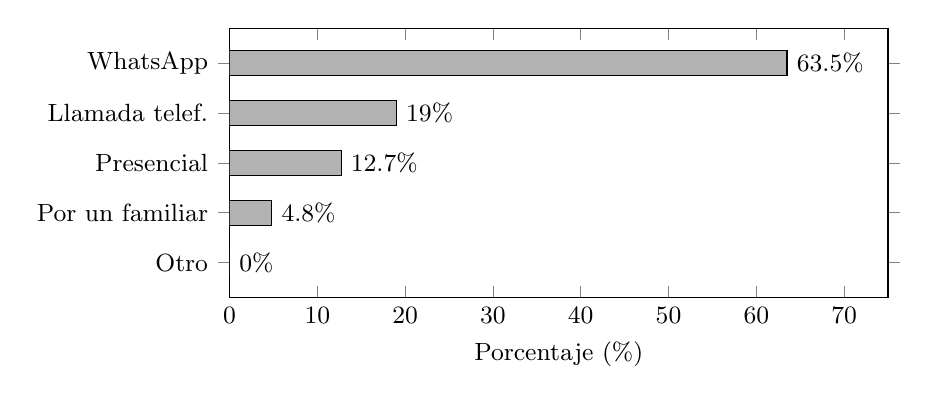
\begin{tikzpicture}
\begin{axis}[
  xbar,
  width=0.82\textwidth, height=5cm,
  bar width=9pt,
  xmin=0, xmax=75,
  xlabel={Porcentaje (\%)},
  ytick={1,2,3,4,5},
  yticklabels={Otro, Por un familiar, Presencial, Llamada telef., WhatsApp},
  ymin=0.3, ymax=5.7,
  nodes near coords={\pgfmathprintnumber[fixed,precision=1]{\pgfplotspointmeta}\%},
  nodes near coords align={horizontal},
  every node near coord/.style={font=\small},
  tick label style={font=\small},
  xlabel style={font=\small},
]
\addplot[fill=gray!60] coordinates {
  (0.0,  1)
  (4.8,  2)
  (12.7, 3)
  (19.0, 4)
  (63.5, 5)
};
\end{axis}
\end{tikzpicture}
\end{center}
\textit{n=40 (63.5\%) WhatsApp; n=12 (19.0\%) Llamada; n=8 (12.7\%) Presencial;
n=3 (4.8\%) Familiar; n=0 (0.0\%) Otro.}

\smallskip
El 63.5\,\% de los pacientes coordinó su última cita mediante WhatsApp, superando en
3.4 veces a la llamada telefónica (19.0\%), segundo canal en frecuencia. La atención
presencial en recepción (12.7\%) y el canal familiar (4.8\%) son residuales. La
concentración en WhatsApp como canal de facto respalda la viabilidad tecnológica de
un asistente automático sobre esa misma plataforma.

% --- Pregunta 2 ---
\medskip
\textbf{Pregunta 2 — Facilidad para encontrar horario disponible (escala 1--5)}

\begin{center}
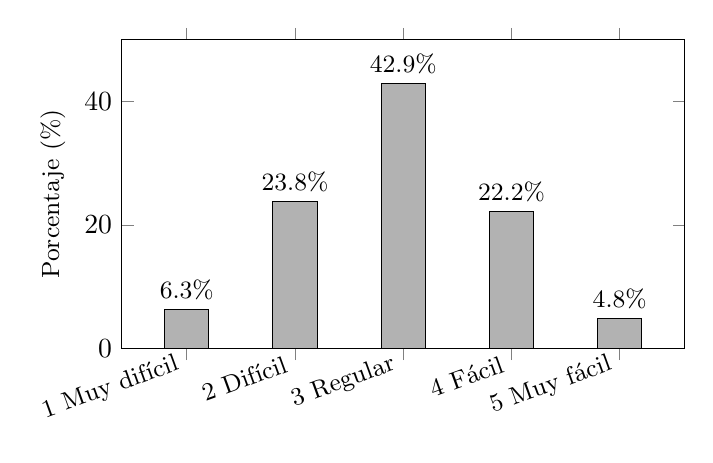
\begin{tikzpicture}
\begin{axis}[
  ybar,
  width=0.72\textwidth, height=5.5cm,
  bar width=16pt,
  ymin=0, ymax=50,
  ylabel={Porcentaje (\%)},
  xtick=data,
  symbolic x coords={1 Muy difícil, 2 Difícil, 3 Regular, 4 Fácil, 5 Muy fácil},
  x tick label style={rotate=20, anchor=east, font=\small},
  nodes near coords={\pgfmathprintnumber[fixed,precision=1]{\pgfplotspointmeta}\%},
  nodes near coords align={vertical},
  every node near coord/.style={font=\small},
  enlarge x limits=0.15,
  ylabel style={font=\small},
]
\addplot[fill=gray!60] coordinates {
  (1 Muy difícil, 6.3)
  (2 Difícil,    23.8)
  (3 Regular,    42.9)
  (4 Fácil,      22.2)
  (5 Muy fácil,   4.8)
};
\end{axis}
\end{tikzpicture}
\end{center}
\textit{n=4 (6.3\%); n=15 (23.8\%); n=27 (42.9\%); n=14 (22.2\%); n=3 (4.8\%).
Media=2.95; Mediana=3; Moda=3; DE$\approx$0.97.}

\smallskip
El 42.9\,\% de los pacientes califica el proceso de agendamiento como ``Regular'', y
al sumar las categorías de dificultad (30.2\%) frente a las de facilidad (27.0\%) la
balanza se inclina hacia la dificultad percibida. La media de 2.95 sobre 5 confirma
que el proceso actual no resulta cómodo para la mayoría.

% --- Pregunta 3 ---
\medskip
\textbf{Pregunta 3 — Situaciones experimentadas con las citas (respuesta múltiple)}

\begin{center}
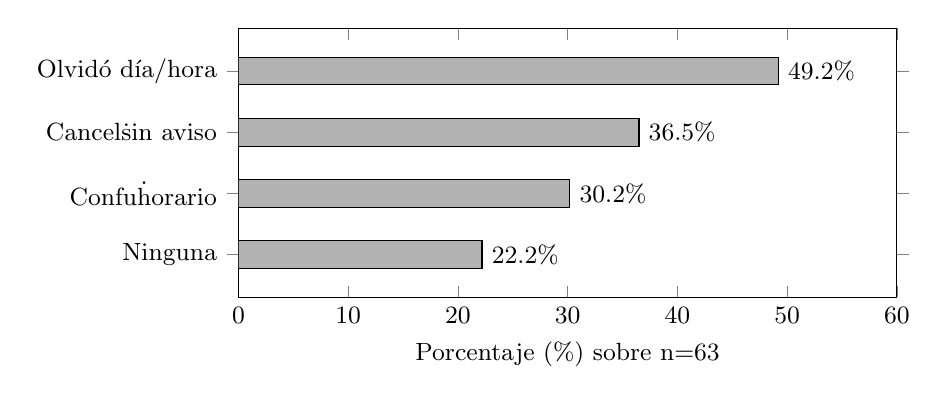
\begin{tikzpicture}
\begin{axis}[
  xbar,
  width=0.82\textwidth, height=5cm,
  bar width=10pt,
  xmin=0, xmax=60,
  xlabel={Porcentaje (\%) sobre n=63},
  ytick={1,2,3,4},
  yticklabels={Ninguna, Confu\. horario, Cancel\. sin aviso, Olvidó día/hora},
  ymin=0.3, ymax=4.7,
  nodes near coords={\pgfmathprintnumber[fixed,precision=1]{\pgfplotspointmeta}\%},
  nodes near coords align={horizontal},
  every node near coord/.style={font=\small},
  tick label style={font=\small},
  xlabel style={font=\small},
]
\addplot[fill=gray!60] coordinates {
  (22.2, 1)
  (30.2, 2)
  (36.5, 3)
  (49.2, 4)
};
\end{axis}
\end{tikzpicture}
\end{center}
\textit{Olvidó día/hora: n=31 (49.2\%); Canceló sin recordatorio: n=23 (36.5\%);
Confundió horario: n=19 (30.2\%); Ninguna: n=14 (22.2\%).}

\smallskip
El 77.8\,\% de los pacientes reportó al menos un incidente relacionado con la gestión
de citas. El olvido del día u hora fue el más frecuente (49.2\%), seguido por
cancelaciones de último momento atribuidas a la ausencia de un recordatorio oportuno
(36.5\%). La proporción de afectados evidencia una necesidad real y generalizada de
un sistema de notificación automática.

% --- Pregunta 4 ---
\medskip
\textbf{Pregunta 4 — Anticipación preferida para el recordatorio automático}

\begin{center}
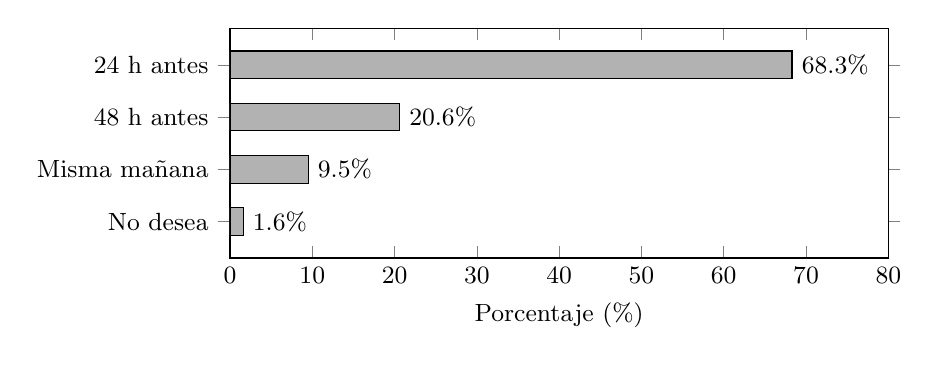
\begin{tikzpicture}
\begin{axis}[
  xbar,
  width=0.82\textwidth, height=4.5cm,
  bar width=10pt,
  xmin=0, xmax=80,
  xlabel={Porcentaje (\%)},
  ytick={1,2,3,4},
  yticklabels={No desea, Misma mañana, 48 h antes, 24 h antes},
  ymin=0.3, ymax=4.7,
  nodes near coords={\pgfmathprintnumber[fixed,precision=1]{\pgfplotspointmeta}\%},
  nodes near coords align={horizontal},
  every node near coord/.style={font=\small},
  tick label style={font=\small},
  xlabel style={font=\small},
]
\addplot[fill=gray!60] coordinates {
  (1.6,  1)
  (9.5,  2)
  (20.6, 3)
  (68.3, 4)
};
\end{axis}
\end{tikzpicture}
\end{center}
\textit{24 h antes: n=43 (68.3\%); 48 h antes: n=13 (20.6\%); Misma mañana: n=6
(9.5\%); No desea: n=1 (1.6\%).}

\smallskip
El 68.3\,\% de los pacientes prefiere recibir el recordatorio 24 horas antes de la
cita, y sumado al 20.6\% que prefiere 48 horas, el 88.9\% de los encuestados se
inclina por un aviso con al menos un día de antelación. Solo el 1.6\% rechaza recibir
recordatorios, lo que indica una aceptación prácticamente universal de la
funcionalidad propuesta.

% --- Pregunta 5 ---
\medskip
\textbf{Pregunta 5 — Gestiones que el paciente desea resolver por WhatsApp
(respuesta múltiple)}

\begin{center}
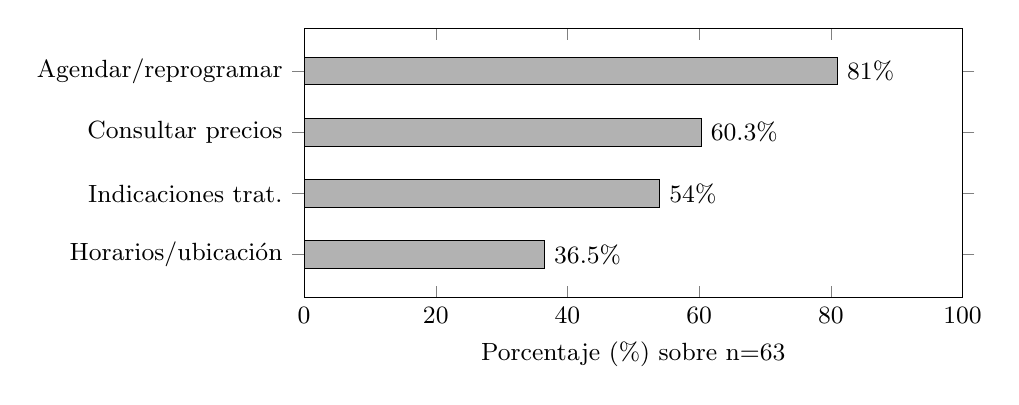
\begin{tikzpicture}
\begin{axis}[
  xbar,
  width=0.82\textwidth, height=5cm,
  bar width=10pt,
  xmin=0, xmax=100,
  xlabel={Porcentaje (\%) sobre n=63},
  ytick={1,2,3,4},
  yticklabels={Horarios/ubicación, Indicaciones trat., Consultar precios, Agendar/reprogramar},
  ymin=0.3, ymax=4.7,
  nodes near coords={\pgfmathprintnumber[fixed,precision=1]{\pgfplotspointmeta}\%},
  nodes near coords align={horizontal},
  every node near coord/.style={font=\small},
  tick label style={font=\small},
  xlabel style={font=\small},
]
\addplot[fill=gray!60] coordinates {
  (36.5, 1)
  (54.0, 2)
  (60.3, 3)
  (81.0, 4)
};
\end{axis}
\end{tikzpicture}
\end{center}
\textit{Agendar/reprogramar: n=51 (81.0\%); Precios: n=38 (60.3\%); Indicaciones:
n=34 (54.0\%); Horarios: n=23 (36.5\%). Promedio de 2.32 funciones seleccionadas
por persona.}

\smallskip
Agendar o reprogramar citas directamente (81.0\%) es la función más demandada por
amplio margen. Le siguen consultar precios y formas de pago (60.3\%) e indicaciones
de tratamiento (54.0\%). En promedio cada paciente marcó 2.32 opciones, lo que sugiere
que el asistente virtual debe ser multifuncional para satisfacer la mayoría de las
necesidades identificadas.

% --- Pregunta 6 ---
\medskip
\textbf{Pregunta 6 — Disposición a interactuar con un asistente virtual (escala 1--5)}

\begin{center}
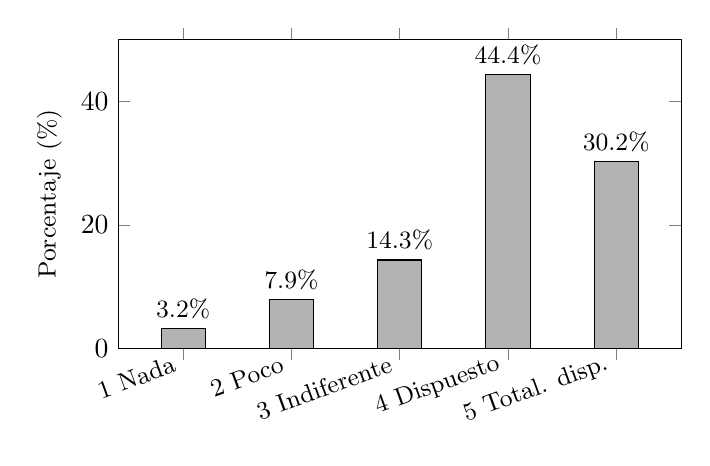
\begin{tikzpicture}
\begin{axis}[
  ybar,
  width=0.72\textwidth, height=5.5cm,
  bar width=16pt,
  ymin=0, ymax=50,
  ylabel={Porcentaje (\%)},
  xtick=data,
  symbolic x coords={1 Nada, 2 Poco, 3 Indiferente, 4 Dispuesto, 5 Total. disp.},
  x tick label style={rotate=20, anchor=east, font=\small},
  nodes near coords={\pgfmathprintnumber[fixed,precision=1]{\pgfplotspointmeta}\%},
  nodes near coords align={vertical},
  every node near coord/.style={font=\small},
  enlarge x limits=0.15,
  ylabel style={font=\small},
]
\addplot[fill=gray!60] coordinates {
  (1 Nada,       3.2)
  (2 Poco,       7.9)
  (3 Indiferente,14.3)
  (4 Dispuesto,  44.4)
  (5 Total. disp.,30.2)
};
\end{axis}
\end{tikzpicture}
\end{center}
\textit{n=2 (3.2\%); n=5 (7.9\%); n=9 (14.3\%); n=28 (44.4\%); n=19 (30.2\%).
Media=3.90; Mediana=4; Moda=4; DE$\approx$1.03.}

\smallskip
El 74.6\,\% de los pacientes se ubica entre ``Dispuesto'' y ``Totalmente dispuesto''
a usar un asistente virtual de WhatsApp, frente a solo el 11.1\% que muestra poca o
nula disposición. Con una media de 3.90 y mediana de 4, la aceptación es alta y
consistente, constituyendo el indicador más sólido de viabilidad de adopción del
canal propuesto.

% ==============================================================
%  INSTRUMENTO 9 — FICHA DE OBSERVACIÓN (PENDIENTE)
% ==============================================================

\paragraph{Resultados de la ficha de observación cronometrada}

El instrumento está diseñado para registrar, mediante observación directa y cronometraje, los tiempos de cada tramo administrativo en las fases de pretest y postest. A continuación se presenta la plantilla del instrumento, cuya aplicación en campo se encuentra pendiente de aprobación por el tutor.

\begin{tcolorbox}[
  enhanced, breakable,
  title={\textbf{Instrumento 9 --- Ficha de Observación Cronometrada}\\
         Tiempo de Gestión Administrativa (OE3) $|$ Centro Odontológico Bellidental},
  fonttitle=\small\bfseries,
  colback=white, colframe=black, colbacktitle=gray!20, coltitle=black,
  boxrule=0.5pt, arc=2pt, left=4pt, right=4pt, top=4pt, bottom=4pt
]
\small
\begin{center}
\textbf{\textit{Observación: la recolección de datos mediante este instrumento se
encuentra pendiente de aprobación por parte del tutor.}}
\end{center}
\vspace{4pt}
Fase: $\square$~Pretest \quad $\square$~Postest \qquad
Fecha: \underline{\hspace{3cm}} \quad
Observador: \underline{\hspace{4cm}} \\[4pt]

\textbf{Datos generales del paciente} \\[2pt]
Tipo de paciente: $\square$~Nuevo \; $\square$~Recurrente \hfill
Hora programada de cita: \underline{\hspace{2.2cm}} \quad
Hora de llegada: \underline{\hspace{2.2cm}} \\[6pt]

\textbf{Tramos administrativos} \\[2pt]
\begin{tabular}{|p{0.44\textwidth}|c|c|c|}
\hline
\textbf{Tramo} & \textbf{Hora inicio} & \textbf{Hora fin} & \textbf{Duración} \\ \hline
T1 — Historia clínica (llenado / actualización) & & & \\ \hline
T2 — Hora inicio atención clínica (referencia) & & & \\ \hline
T3 — Hora fin atención clínica (referencia) & & & \\ \hline
T4 — Registro post-consulta (receta, actualización) & & & \\ \hline
T5 — Registro de pago \newline
(¿Consulta de saldo? Sí \,$\square$ \; No \,$\square$) & & & \\ \hline
T6 — Agendamiento próxima cita & & & \\ \hline
\end{tabular} \\[6pt]

\textbf{Indicadores calculados} \\[2pt]
Tiempo administrativo total $(T_1 + T_4 + T_5 + T_6)$: \underline{\hspace{3cm}} \\
Retraso vs.\ cita programada $(T_2 - \text{Hora programada})$: \underline{\hspace{3cm}} \\
Espera tras llegada $(T_2 - \text{Hora de llegada})$: \underline{\hspace{3cm}} \\[4pt]

\textbf{Incidencias observadas:} \\
\underline{\hspace{\linewidth}} \\
\underline{\hspace{\linewidth}} \\
\underline{\hspace{\linewidth}}
\end{tcolorbox}

\paragraph{Fichas de contenido documental}

Para sustentar teóricamente el diseño del sistema, se revisaron trabajos científicos relacionados con arquitecturas de microservicios, sistemas de información odontológica y agentes conversacionales en salud. Las fichas siguientes sintetizan las fuentes más relevantes, destacando sus ideas centrales y el aporte específico al presente estudio.

\begin{table}[htbp]
    \caption{Ficha de contenido documental: Arcila-Díaz \& Valdivia (2022)}
    \label{tab:ficha_arcila_2022}
    \renewcommand{\arraystretch}{1.4}
    \begin{tabularx}{\textwidth}{@{}>{\bfseries}p{4.2cm} X@{}}
        \toprule
        Campo & \textbf{Descripción} \\
        \midrule
        Tema & Arquitectura de software orientada a microservicios para la disponibilidad e integración de registros de salud dental. \\
        Año de publicación & 2022 \\
        Referencia bibliográfica & J. Arcila-Diaz and C. Valdivia, ``A Microservice-based Software Architecture for Improving the Availability of Dental Health Records,'' \textit{International Journal of Computing}, vol.~21, no.~4, pp.~475--481, 2022, doi: 10.47839/ijc.21.4.2783. \\
        Ideas centrales & Propuesta y validación experimental de una arquitectura distribuida mediante microservicios desacoplados para centralizar registros odontológicos bajo normativas sanitarias, garantizando alta disponibilidad, seguridad por tokens y escalamiento independiente frente a la fragmentación de datos clínicos. \\
        Conceptos clave & Arquitectura de microservicios, API Gateway, API REST, autenticación JWT, disponibilidad de historias clínicas, pruebas de carga (JMeter). \\
        Conclusiones & La descomposición por dominios funcionales acoplada a un API Gateway soporta hasta 21 solicitudes por segundo por instancia con 100\% de disponibilidad, optimizando el rendimiento computacional sin exponer directamente las bases de datos internas. \\
        Aporte al tema & Sustenta la arquitectura backend del sistema centralizado: separación de dominios (pacientes, citas, registros clínicos), uso de API Gateway como punto único de integración desacoplado para el agente conversacional y control de acceso mediante tokens. \\
        Observaciones & Estudio enfocado estrictamente en atributos de calidad de software (rendimiento computacional y disponibilidad); no evalúa tiempos de gestión administrativa humana ni integra canales de mensajería automatizada. \\
        \bottomrule
    \end{tabularx}
\end{table}

\begin{table}[htbp]
    \caption{Ficha de contenido documental: Alejandrino \& Pajota (2023)}
    \label{tab:ficha_alejandrino_2023}
    \renewcommand{\arraystretch}{1.4}
    \begin{tabularx}{\textwidth}{@{}>{\bfseries}p{4.2cm} X@{}}
        \toprule
        Campo & \textbf{Descripción} \\
        \midrule
        Tema & Sistema de información para clínicas dentales privadas con integración de un sistema de chatbot. \\
        Año de publicación & 2023 \\
        Referencia bibliográfica & J. C. Alejandrino and E. L. P. Pajota, ``An Information System for Private Dental Clinic with Integration of Chat-Bot System: A Project Development Plan,'' \textit{International Journal of Advanced Trends in Computer Science and Engineering}, vol.~12, no.~2, pp.~38--43, 2023, doi: 10.30534/ijatcse/2023/011222023. \\
        Ideas centrales & Planificación de un sistema centralizado web para reemplazar registros manuales en clínicas odontológicas, integrando un agente conversacional para la reserva de citas y proyectando una disminución del 68.75\% en el tiempo total de gestión administrativa (de 80 a 25 minutos en tareas clave). \\
        Conceptos clave & Arquitectura web cliente-servidor, chatbot basado en reglas con procesamiento de lenguaje natural (NLP), automatización del agendamiento, APIs de integración, optimización del tiempo administrativo. \\
        Conclusiones & La integración modular de historias clínicas, facturación y un chatbot conversacional mitiga cuellos de botella y reduce los tiempos de espera y procesamiento operativo en entornos dentales privados. \\
        Aporte al tema & Aporta una referencia directa sobre la arquitectura modular (administración, citas y reportes), el diseño lógico del chatbot con NLP para agendamiento automatizado y un desglose metodológico de tiempos de proceso análogo al flujo clínico evaluado. \\
        Observaciones & Estudio de nivel conceptual/plan de desarrollo; las reducciones temporales constituyen estimaciones de diseño y no mediciones empíricas posimplementación. \\
        \bottomrule
    \end{tabularx}
\end{table}

\begin{table}[htbp]
    \caption{Ficha de contenido documental: Santhosh et al. (2026)}
    \label{tab:ficha_santhosh_2026}
    \renewcommand{\arraystretch}{1.4}
    \begin{tabularx}{\textwidth}{@{}>{\bfseries}p{4.2cm} X@{}}
        \toprule
        Campo & \textbf{Descripción} \\
        \midrule
        Tema & Agente conversacional basado en inteligencia artificial integrado a WhatsApp para la gestión de citas médicas. \\
        Año de publicación & 2026 \\
        Referencia bibliográfica & Santhosh and Sanath Kumar Team, ``Healthcare Appointment Booking On Whatsapp By Using AI Agent,'' Parul University, preprint, 2026, doi: 10.13140/RG.2.2.28074.99520. \\
        Ideas centrales & Implementación de un agente conversacional para automatizar el ciclo integral de citas médicas (reserva, reprogramación y cancelación) mediante mensajería instantánea, reduciendo el tiempo operativo de reserva de un rango de 5--8 minutos a 3 minutos y 42 segundos en pruebas con usuarios reales. \\
        Conceptos clave & WhatsApp Cloud API, modelos de lenguaje grande (LLM), orquestación de flujos de trabajo (n8n), máquina de estados finita, optimización del tiempo de reserva. \\
        Conclusiones & La orquestación de un LLM acoplado a una API de mensajería mitiga las rigideces del software tradicional, resolviendo un 68\% de las consultas administrativas y alcanzando un 96.2\% de precisión en la detección de intenciones operativas. \\
        Aporte al tema & Proporciona un patrón arquitectónico directo para el agente conversacional: integración vía webhooks, manejo del diálogo mediante máquina de estados y estructuración de respuestas en formato JSON acotadas al dominio clínico. \\
        Observaciones & Estudio aplicado con validación preliminar en entorno ambulatorio (UAT, $n = 40$); no evalúa la integración previa con sistemas de historias clínicas ni incluye un grupo de control formal. \\
        \bottomrule
    \end{tabularx}
\end{table}
